\chapter{Wavelet Gain Layer Additional Results}\label{app:ch6:more_results}
\def \path {freqlearn/}
\def \imgpath {freqlearn/images}
This appendix presents some additional results for the gain layer experiments
from \autoref{sec:ch6:ablation}. Here, we do ablation experiments similar to
those done on the invariant layer in \autoref{sec:ch5:conv_exp}. In particular,
we use the architecture described in \autoref{tab:ch5:cifar_tiny_arch} and
progressively swap out convolutional layers with gain layers. 
Again, we run this on CIFAR-10, CIFAR-100 and Tiny ImageNet. 

We use the same naming technique as in the previous chapter, calling a network
`gainX' means that the `convX' layer was replaced with a wavelet gain layer, but
otherwise keeping the rest of the architecture the same. Recall that the
CIFAR architectures in \autoref{tab:ch5:cifar_tiny_arch} have 6 convolutional layers 
called `convA' to `convF', and the Tiny ImageNet architectures have 8
convolutional layers called `convA' to `convH'.

We train all our networks for with stochastic gradient descent with momentum.
The initial learning rate is $0.5$, momentum is $0.85$, batch size $N=128$ and
weight decay is $10^{-4}$. For CIFAR-10/CIFAR-100 we scale the learning rate by
a factor of 0.2 after 60, 80 and 100 epochs, training for 120 epochs in total.
For Tiny ImageNet, the rate change is at 18, 30 and 40 epochs (training for 45 in total).

\autoref{fig:app6:gl_results} and \autoref{fig:app6:gl_results_ti} show the results 
from these experiments for CIFAR and Tiny ImageNet. Just as with the large
kernel ablation study in \autoref{sec:ch6:ablation}, adding a gain layer
typically degrades performance by a small amount.

\begin{figure}[t]
  \centering
  \subfloat[CIFAR-10]{%
    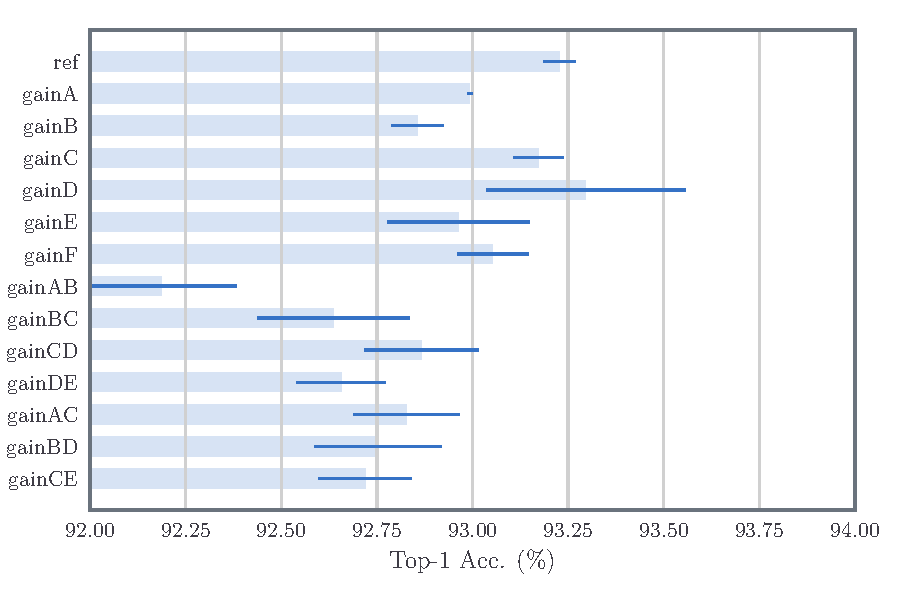
\includegraphics[width=\textwidth]{\imgpath/cifar10_gainlayer.pdf}
    \label{fig:app6:cifar10_gl}
  }\\
  \subfloat[CIFAR-100]{%
    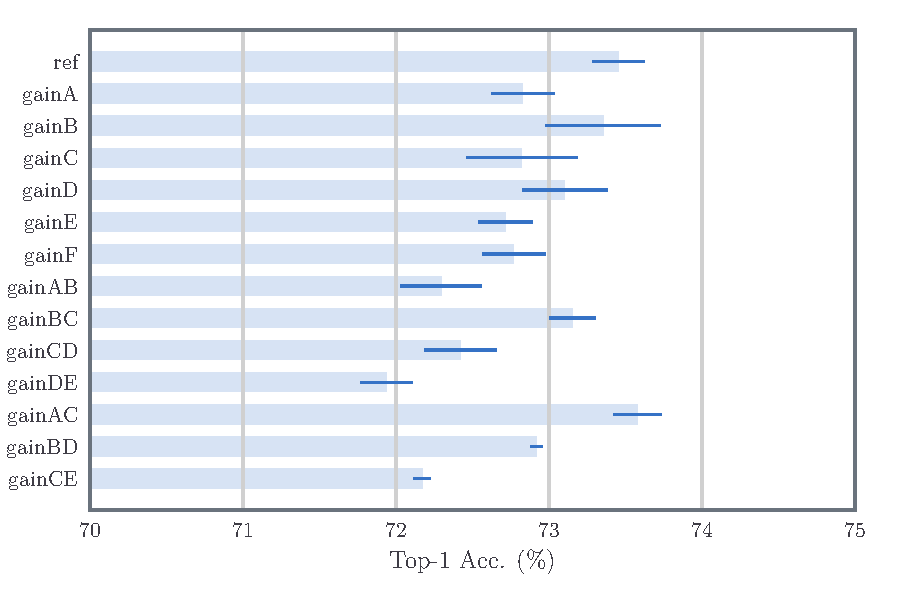
\includegraphics[width=\textwidth]{\imgpath/cifar100_gainlayer.pdf}
    \label{fig:app6:cifar100_gl}
  }
  % \subfloat[Tiny ImageNet]{%
    % 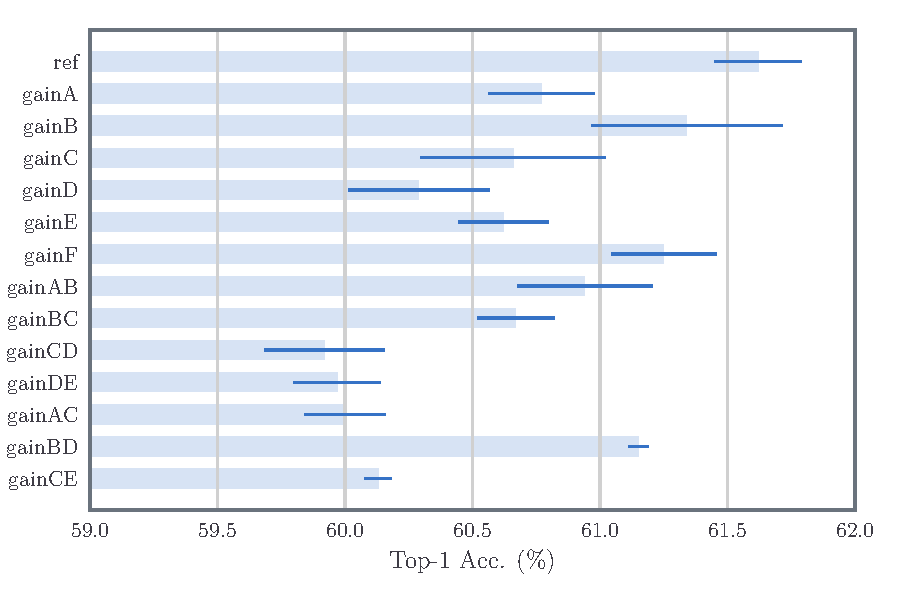
\includegraphics[width=0.8\textwidth]{\imgpath/ti_gainlayer.pdf}
    % \label{fig:ch6:ti_gl}
  % }\\
  \mycaption{Small kernel ablation results for CIFAR}{These graphs show the
  average and $\pm 1$ standard deviation results for 3 runs. The names on the
  left represent where the convolutional layer is swapped for a gain layer, with
  `gainAB' and below indicating two convolutional layers were swapped for gain
  layers.}
  \label{fig:app6:gl_results}
\end{figure}

\begin{figure}[t]
  \centering
  \subfloat[Tiny ImageNet]{%
    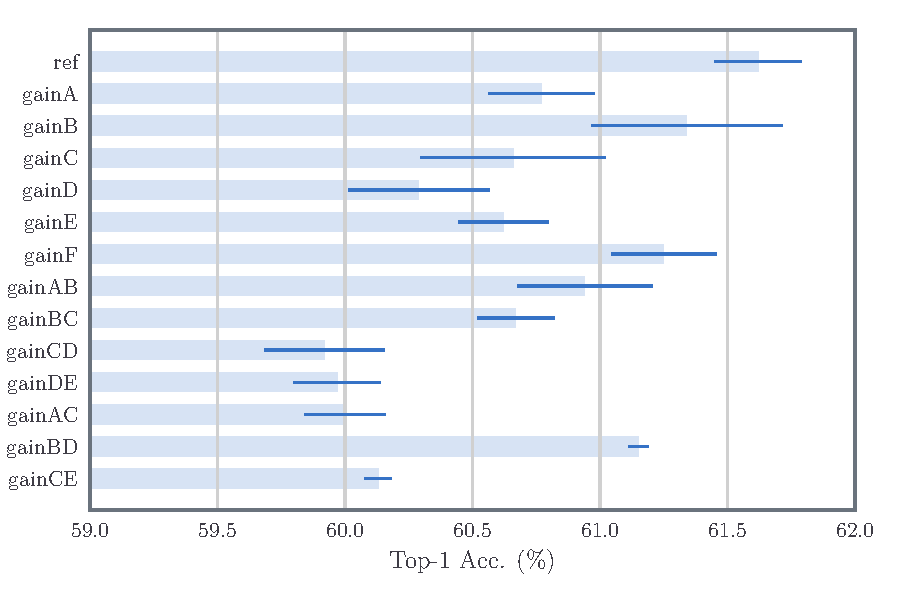
\includegraphics[width=\textwidth]{\imgpath/ti_gainlayer.pdf}
    \label{fig:app6:ti_gl}
    }
  % \subfloat[Tiny ImageNet]{%
    % 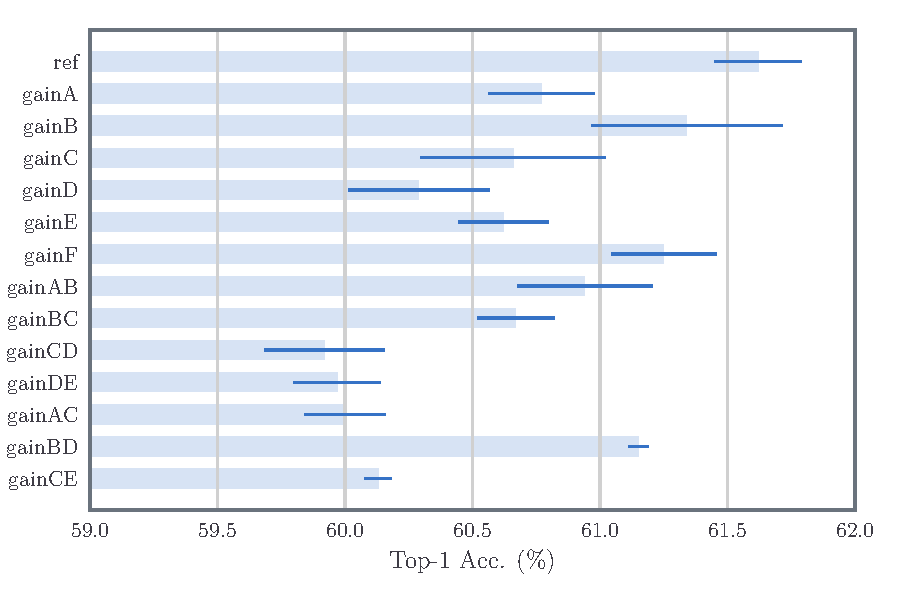
\includegraphics[width=0.8\textwidth]{\imgpath/ti_gainlayer.pdf}
    % \label{fig:ch6:ti_gl}
  % }\\
    \mycaption{Small kernel ablation results for Tiny ImageNet}{}
  \label{fig:app6:gl_results_ti}
\end{figure}


